\documentclass{beamer}

\usepackage{beamerthemesplit}

\title{Carbon Nanotube software: TubeBuilder}
\date{\today}
\author{Spencer Krum, Miach Eastman, Dr. Jun Jaio}

\begin{document}

\frame{\titlepage}

% Slide 
\section{Introduction}
\subsection{Overview}
\frame 
{
    \frametitle{The research}
    \begin{itemize}
        \item Carbon Nanotube Software
        \item Simulate Real Tubes
        \item From Experimental Data
        \item Curved Tubes
        \item Open Source
    \end{itemize}
%%    \textbf{2009}
%%    \begin{itemize}
%%        \item Amen Kester
%%        \item Art Aldridge
%%        \item Jeff Doghety
%%    \end{itemize}
%%    \textbf{2010}
%%    \begin{itemize}
%%        \item Greg Haynes
%%        \item Patrick Bledsoe, Connor O'Connel,  Kris Sims, Amber Lauer, Shar Smith, Sammie Page, Spencer Krum, Jeff Doughtey
%%        \item Keith Parker, Philip Witham, Kristine Summerfield
%%        \item \textbf{Faculty:} Dr. Erik S\'anchez, Dr. Bart Massey
%%    \end{itemize}
}

%\subsection{Sponsors}
%\frame
%{
%    \frametitle{A really, really big thankyou}
%    \begin{columns}[t]
%    \column{.5\textwidth}
%    \begin{itemize}
%        \item Bill Feyerherm
%        \item Erik S\'anchez
%        \item Sunstone Circuits
%        \item TAP Plastics
%        \item Derek Nowak
%        \item Jane Bloom
%        \item Dept. of Physics
%        \item Bart Massey
%        \item Parallax
%        \item Hoffman Construction
%        \item SolidWorks
%    \end{itemize}
%    \column{.5\textwidth}
%    \begin{itemize}
%        \item Free Geek
%        \item Drake Mitchel
%        \item Eric Bodegom
%        \item The CAT
%        \item Society of Physics Students
%        \item Allison Whited
%        \item Suzzane Flores
%        \item Masseh College of Engineering and Computer Science?
%    \end{itemize}
%    \end{columns}
%}

%%%%%%\subsection{A bit of history - 2009}
%\frame
%{
%    \frametitle{ROV 2009}
%
%{\bf PSU-ROV 2009}
%{\it Total UROV cost: \$481.10}
%
%In 2009, the Portland State University ROV team sent three students and one mentor to Boston, Massachusetts, where the underwater vehicle did not pass the safety inspection due to unforeseen electrical difficulties. The robot was unable to participate in the competition. The team received 0/300 mission points and 80.67/500 for the total score(mostly for the technical report), ranking 28th. 
%
%}
%
%\subsection{A bit of history - 2010}
%\frame
%{
%    \frametitle{ROV 2010}
%    
%
%\noindent
%{\bf PSU-ROV 2010}
%{\it Total UROV cost: \$2496.06}
%
%In June of 2010, the Portland State Robotics Team completed an underwater remotely operated vehicle (UROV) to compete in the Marine Advancement for Technology Education (MATE) Center's annual international competition. Out of over four hundred applicants for the combined competition classes, the Portland Sate University ROV team passed the local qualification round and went on to participate in the international competition. 
%Five students and two mentors went to Hilo, Hawaii to compete. The 2010 ROV received 70/300 mission points and 216/500 total points, 
%ranking 18th out of 26 international teams. The team learned and demonstrated the ability to produce a working machine under budget and time constraints.
%
%}
% Slide
\subsection{Demo example}
\frame
{
    \frametitle{Demo}
    \begin{itemize}
        \item Demo
    \end{itemize}
}

% Slide
\section{How it works}
\subsection{Popov}
\frame
{
    \frametitle{How a tube rolls up}

    \begin{center}
    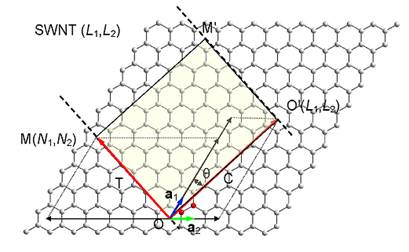
\includegraphics[width=1\textwidth]{grid.jpg}
    \end{center}
}

\subsection{Popov}
\frame
{
    \frametitle{t-vectors}

    \begin{center}
    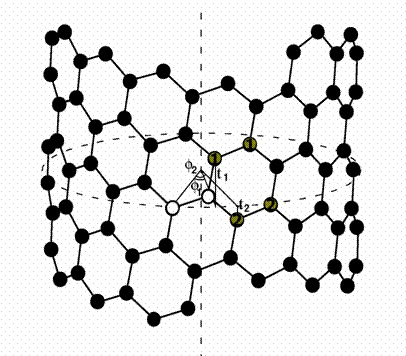
\includegraphics[width=1\textwidth]{tvectors.jpg}
    \end{center}
}
%%%%% Slide
%%%%\subsection{Example Installation}
%%%%\frame
%%%%{
%%%%    \frametitle{Example Secret Installation}
%%%%    \includegraphics[width=1\textwidth]{example_base.png}
%%%%    
%%%%}    
% Slide

\subsection{Code Tour}
\frame
{
    \frametitle{RTFS!}
    \begin{center}
    RTFS!
    \end{center}
}

%Slide
\section{Thanks}
\subsection{You are awesome}
\frame
{
    \frametitle{Thank you!}
    Thanks to:

    \begin{itemize}
        \item PSU Physics
        \item REU Program
        \item Dr. Jaio
        \item Devon Mcclain
        \item James Hoffman
    \end{itemize}
    
}
\end{document}

